\section{INTRODUCTION}

\begin{figure}
\begin{center}
  \begin{tabular}{@{\hspace{0.1cm}}c}
		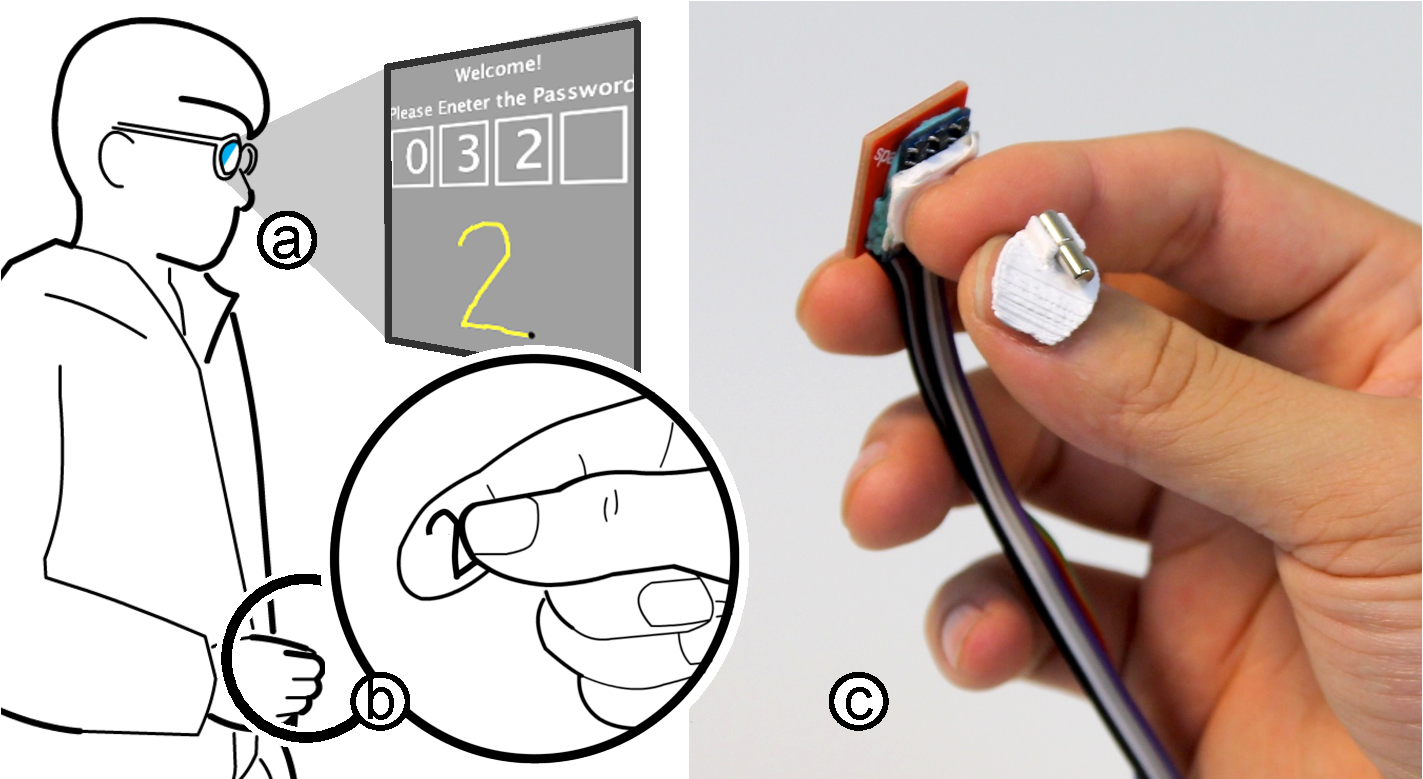
\includegraphics[width=1\linewidth]{firstFigure7}\\
   \end{tabular}
\caption{FingerPad enables touchpad function through the pinched fingertips using magnetic tracking, by adding a magnet and hall sensors on the fingernails, allowing for private and rich subtle interactions. Here, the user enters passwords to the (a) private glass display by (b) drawing numbers with the thumb tip on the index fingertip.}
\label{fig:firstFigure}
\end{center}
\end{figure}

%Human fingers allow for precise grasp of highest dexterity. This ability is a key to fine control of small tangibles. For instance, a small tangible pinched between thumb and fingers allows for arbitrary control of three-dimensional orientation.
%for grasping operations human hand has a high number of degrees of freedom, and there are many grasping styles depending on the shape of an object and purpose. 

Recent development in mobile computing proposes glass-mounted displays. 
Though similar to head-mounted displays, glass-mounted displays (e.g., Google Glass) are specially designed to be light-weighted, attachable, nonobstructive to natural vision, and with increased social acceptance. 

Although displays of this kind allow for personal and private visual outputs, their input methods may not keep the same level of privacy.
Voice input, for example, is commonly used for glass-mounted displays because it is expressive and effective. However, voice input can be problematic in loud environment, and inappropriate in public space when privacy is required (e.g., password input) \cite{Sawhney:2000}. 
Gesture input receives the similar privacy concern, because the input behaviors are easily observable.

%Subtle interactions rely on implicit movement as input, and are generally considered social acceptable. 

To allow for private input, recent research proposes subtle interactions \cite{Costanza:2007}\cite{Saponas:2009}\cite{wolf2011microinteractions}, which looks upon implicit movements and are generally considered socially acceptable. 
For example, muscle interface \cite{Saponas:2009} allows to input through unobservable muscle movement.
Foot gesture \cite{Scott:2010} detects subtle foot motions.
Ring devices \cite{Ogata:2012, Ashbrook:2011} and fabrics \cite{Karrer:2010} are developed to support tapping, spin, and slider inputs. %subtle and socially acceptable.
Although these methods allow subtle inputs (thus, private and socially acceptable), they generally suffered from limited input space.

%Input through implicit foot gestures \cite{Scott:2010} are not easily observable. 
%Input through finger rings \cite{Ogata:2012, Ashbrook:2011} or pinch fabrics \cite{Karrer:2010} are subtle and also socially acceptable.


% and are generally considered socially acceptable
%Foot gestures \cite{Scott:2010} are not easily observable. 
%Ring devices are developed to support tapping and spin input \cite{Ogata:2012, Ashbrook:2011}.
%Pinched fabrics \cite{Karrer:2010} allows for 1D slider input.


%Pinstripe \cite{Karrer:2010} allows 1D slider through pinched fabrics.
%or by implicitly move some body parts \cite{Scott:2010}.


%To allow for private input, researchers proposes subtle interactions \cite{Saponas:2009}\cite{wolf2011microinteractions}.


%In addition to privacy, social acceptance is another concern for the input methods. 
%Recent research proposes subtle interactions \cite{Saponas:2009}\cite{wolf2011microinteractions}.

%input through fabrics

%, not easily extensible for rich interactions. 



%previous subtle interactions only allows for limited input space, not easily extensible for rich interactions. 

%Subtle interactions \ref{Saponas:2009} are proposed as the mean to mitigate this concern.




% readily available
%There are situations where users were intended to access user controls at given posture. For instance, lying in bed, the user waken by an alarm strugglingly searches for the phone to set-off. This requires the effort to retrieve the devices (e.g., the phone). Always-available input \ref{Saponas:2009}[N] mitigates this effort by moving user controls to wearable devices which are easily accessible. 

%By removing this effort, users can save time and reduce errors (where is the error?).

% pinch gesture is natural.  ready for input.

% finger-worn device maximize availability / accessibility

%Instrumenting devices around fingers maximize the accessibility.

%even useable in no-hand situation

%Finger-worn device

%availability

%Always-available input \ref{Saponas:2009}[N] mitigates this effort by moving user controls to wearable devices which are easily accessible. 

% minimal travel distance, but not allowing rich interaction 
%Nevertheless, not all wearable devices are readily available. This availability depends on the effort to reach to the device controls. 
%To reduce this distance, previous works implement input functions around the users' hands. (Armtech) MuscleInput \ref{Saponas:2009}, for example, allows the wrist bend devices to read muscles movement as input. (FingerTech) Finger ring devices are developed to support tapping [iRing], 1D rolling \ref{Ashbrook:2011}, and marking menus through the ring.  These methods allow to input with little efforts, but provide limited input space, not easily extensible for rich interactions. 

%Wrist-watch touch screens, for example, require users hands traveling to the touchscreen, which introduces efforts. Gesture inputs \ref{Rekimoto:2001}\ref{Kim:2012} effectively increase availability with zero travel distance, but requires users to memorize functional mappings. 


%To support complex inputs, touch-based watch-display seems  a feasible solution, nevertheless, requiring the effort to reach to the touch screen.

%here, highlight strength of FingerPad.
%reach to FingerPad is a pinch-away. 


%\subsubsection{FingerPad}



%Benefits of FingerPad
We present FingerPad, a nail-mounted device that turns pinched fingertips into a touchpad, allowing for private and rich subtle interactions. As illustrated in Figure \ref{fig:firstFigure}, the user treats the index fingertip as the touchpad, and the thumb as the touch stylus.
FingerPad enables the touchpad function using magnetic tracking, by adding a magnet and hall sensors on the fingernails. 
Functionally, FingerPad is equivalent to a touchpad that users can learn with minimal effort.  Allowing for 2D touch inputs, FingerPad is ready for rich interactions including pointing, marking menu, and stroke input. 

%Unlike touchpads where fingers are styluses, FingerPad could interpret a finger pinch as the thumb touching the index fingertip (e.g., thumb as stylus, and index fingertip as touchpad), and vice versa. In this work, we identify two primary uses of FingerPad, namely IndexPad and ThumbPad. The two models both exist, and only in users� heads. Wrong model applied in FingerPad leads to inverted interpretation of touch positions. In the explorative study, we found the model applied in users� heads is related to the context of use, and highly affected by their experience in using touchpads. One primary factor is the orientation of fingers in use of FingerPad. For example,  touchpads typically faces up that fingers can effortlessly touch down. We will discuss more details in the study section.

%The rest of the paper is arranged as follows. First, related work is discussed. Then, the design of FingerPad is introduced and several example applications are presented to illus trate the enabled design space. Then, the underlying mechanism is detailed, including an evaluation and an examination of limitations, and the feedback of users, gathered from the explorative study is presented. Finally, conclusions are drawn and directions of future work suggested. 

\subsubsection{Benefits and limitations}
Allowing for touchpad functions through the fingers in pinch suggests several benefits. (1) Private: the movements of the fingers in pinch are subtle and naturally occluded by the operation hand. (2) Rich: the touchpad function allows input techniques, such as pointing, marking menu and stroke input. (3) Eyes-free: users can perform pinch gestures without visual support. (4) Natural haptic feedback:  by attaching on the nails, we preserve the natural haptic feedbacks on the fingertips, not affecting native functions of fingertips (e.g., grip small objects).
Additionally, by tracking through magnetism, FingerPad is occlusion free (i.e., can use with hand in pocket).


